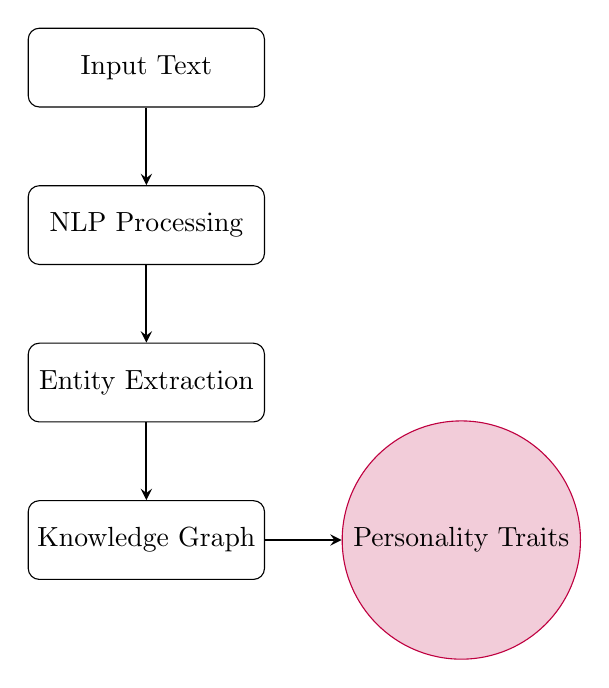
\begin{tikzpicture}[node distance=2cm]
% Define styles
\tikzstyle{entity} = [rectangle, rounded corners, minimum width=3cm, minimum height=1cm, text centered, draw=black]
\tikzstyle{trait} = [circle, draw=purple, fill=purple!20, minimum size=1.5cm]
\tikzstyle{arrow} = [thick,->,>=stealth]

% Draw nodes
\node (text) [entity] {Input Text};
\node (nlp) [entity, below of=text] {NLP Processing};
\node (entities) [entity, below of=nlp] {Entity Extraction};
\node (kg) [entity, below of=entities] {Knowledge Graph};
\node (personality) [trait, right of=kg, xshift=2cm] {Personality Traits};

% Draw arrows
\draw [arrow] (text) -- (nlp);
\draw [arrow] (nlp) -- (entities);
\draw [arrow] (entities) -- (kg);
\draw [arrow] (kg) -- (personality);

\end{tikzpicture}